\documentclass{standalone}
\usepackage{tikz}
\usetikzlibrary{positioning}
\usetikzlibrary{decorations.pathmorphing}

\tikzset{snake it/.style={decorate, decoration={snake, segment length=1.5mm, amplitude=0.5mm}}}
\tikzset{
    position/.style args={#1:#2 from #3}{
        at=(#3.#1), anchor=#1+180, shift=(#1:#2)
    }
}

\begin{document}
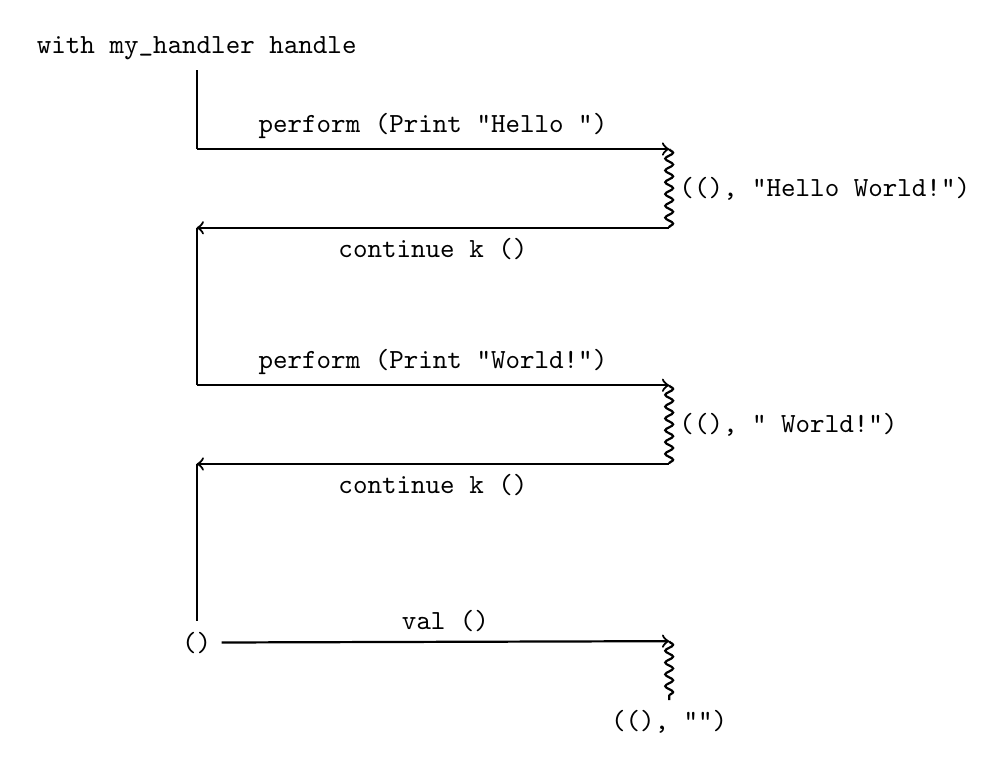
\begin{tikzpicture}
    \draw[thick] (0, 0) -- (0, -1)
        node[at start, above]{\verb|with my_handler handle|};
    \draw[->, thick] (0, -1) -- (6, -1)
        node[midway, above]{\verb|perform (Print "Hello ")|};
    \draw[thick, snake it] (6, -1) -- (6, -2)
        node[right, midway]{\verb|((), "Hello World!")|};
    \draw[->, thick] (6, -2) -- (0, -2)
        node[midway, below]{\verb|continue k ()|};
    \draw[thick] (0, -2) -- (0, -4);
    \draw[->, thick] (0, -4) -- (6, -4)
        node[midway, above]{\verb|perform (Print "World!")|};
    \draw[thick, snake it] (6, -4) -- (6, -5)
        node[right, midway]{\verb|((), " World!")|};
    \draw[->, thick] (6, -5) -- (0, -5)
        node[midway, below]{\verb|continue k ()|};
    \draw[thick] (0, -5) -- (0, -7)
        node[at end, below](UNIT){\verb|()|};
    \draw[->, thick] (UNIT) -- (6, -7.25)
        node[midway, above]{\verb|val ()|};
    \draw[thick, snake it] (6, -7.25) -- (6, -8)
        node[below, at end]{\verb|((), "")|};
    
    
    % \draw[help lines] (0,0) grid (10,-10);
\end{tikzpicture}
\end{document}